\documentclass[Main.tex]{subfiles} 
\begin{document}

\subsubsection{Use Case 3: Vis tid for n�rmeste bus for valgt stoppested}

Use casen kan initialiseres efter Use Case 2 er fuldf�rt. N�r et stoppested trykkes, s�ttes stoppestedsnavnet i den �verste informations bar p� viewet. Desuden s�ttes teksten i begge endestationsbokse til "Loading", og tiden s�ttes til "nn:nn:nn". Herefter unders�ges der f�rst om der er net. Hvis der er, unders�ges der om et stoppested allerede er valgt, og dermed om Use Case 3 allerede er igang, og hvis der er, interruptes tr�den. N�r tr�den er helt lukket, kaldes "GetBusTime" i TrackABusProvideren med rutenavnet, det valgte stoppested samt en ny MessageHandler som parametrer\\
"GetBusTime" st�r for at hente tiden og endestationen for den n�rmeste bus, i begge retninger p� ruten. Udregningen af dette ligger som en stored procedure p� MySQL databasen. Dette kan l�ses om i afsnit \textit{9.1.3: Stored Procedures}. N�r udregningerne er f�rdige, returneres resultaterne til TrackABusProvideren, hvor de bliver pakket ned i en Message, og sendt til MessageHandleren. MessageHandleren ligger i BusMapActivity, og s�rger for at opdatere viewet. Hvis der ikke er nogen bus, som k�rer mod stoppestedet i en eller begge retninger, retuneres der "anyType{}" i den relevante retnings endesstations v�rdi. Hvis en eller begge endestations resultater er denne v�rdi, opdateres endestations teksten til  "No bus going in this direction" og tiden til "nn:nn:nn", for den relevante retning. Hvis endestations teksten i forvejen er "No bus going in this direction", opdateres der intet for den givne retning. Grunden til endestations v�rdien opdateres er, at en rute kan v�re kompleks med mere end to endestation, og en given bus, kan k�re p� samme ruten som en anden bus, men ikke have samme endestation.\\
\\Hvis tilgangen til internettet forsvinder efter et stoppested er valgt, vil opdateringstr�den stadig k�re, men der vil blive vist en besked om, at tiden ikke l�ngere holdes opdateret. Herved, n�r forbindelsen genetableres, forts�ttes tidsopdateringen p� ny. N�r BusMapActivity g�r i dvale s�ttes opdateringstr�den p� pause, og ved gen�bning startes tr�den igen.
P� figur \ref{fig:UC3SSD} kan et simpelt sekvensdiagram for forl�bet ses. Diagrammet viser en hentning af tiden og endestationer i begge retninger, hvor hentningen antages at v�re succesfuld.

\begin{figure}[H]
	\centering
	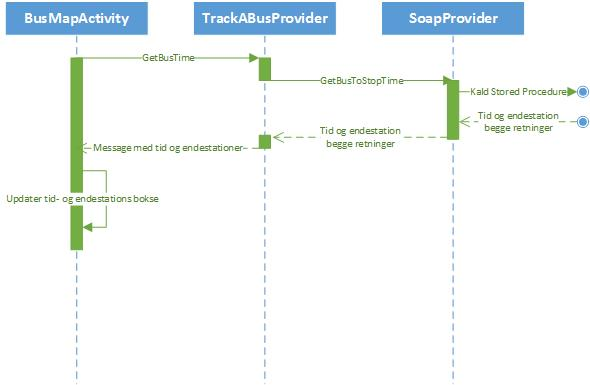
\includegraphics[scale=0.65]{Diagrammer/Sekvensdiagrammer/UC3SSD}
	\caption{Sekvensdiagram for hentning af endestationer og tid for n�rmeste bus.}
	\label{fig:UC3SSD}
\end{figure}




\end{document}